\chapter{Results}
\label{chapter:results}

In this chapter the results of the study will be presented. First the limited liability housing company board member interview results are presented. Then the researcher presents the results gained from customer journey mapping which was done together with energy company and. Lastly, the researcher presents the results from the prototypes and tests conducted during the research. 

\section{Limited Liability Housing Company Board Member Interview Results}
\label{section:interviews}
In this chapter the results of the interviews are discussed and presented by the themes found in the analyzing. The themes are motivation of the board, role of the deputy landlord, overall decision making in a housing company, identified board types and awareness of energy efficiency.

\subsection{Motivation of the Board}

Motivation of the board was discovered to be the biggest factor affecting the actions of a board of the housing company. Based on the interviews, the reasons why people are part of the board and what kind of people they are affects the motivation and operation of the board.

\subsubsection*{Reasons to be in the Board}

The reasons why people are in the board of housing companies varies and it is not the same for everyone but usually the reasons are overlapping and connected to each other. The following themes were identified as reasons to be part of the board:
\begin{itemize}
	% You can use this command to set the items in the list closer to each other
	% (ITEM SEParation, the vertical space between the list items) 
	\setlength{\itemsep}{1pt}
	\item Take care of the value of the investment.
	\item Make sure that things are done correctly.
	\item Personality and experience of the people.
	\item Other people persuade.
	\item Desire to make housing company better and modern.
\end{itemize}

The main reason found out was that the members of the board want to take care of the investment's value they have made when buying the apartment. This reason is based on the fact that living in a detached house is basically the same thing as living in an apartment house and both of them needs maintenance in the same way.

\begin{displayquote}
\textit{I had a bigger risk to loose my money if I didn't go there (to the board). I wanted to make sure that the traditional pipe repair will come and that it will get done.} --- interviewee
\end{displayquote}

\begin{displayquote}
\textit{I also do not understand what is so difficult that people do not want (to go to the board). I find it really important that it is my property and it needs to be treated well. -- The apartment building requires care as well as a detached house.} --- interviewee
\end{displayquote}

Taking care of the investment's value is connected to the fact where the people want to make sure that the things are done with care and correctly. This can be the case even though there is no investment made on behalf of the board member. One interviewee who did not live in the building was part of the board because of his relative was living in the building and he wanted to make sure that the good living conditions were guaranteed and that the things run smoothly in the housing company.

\subsubsection*{Background and Personality of the People}

From the interviews it was also clear that personality and background of the people play a role in why people go to the board. Some of the interviewees felt responsibility to be in the board since no one else had volunteered. In some cases this responsibility is also connected to the need of taking care of the investment's value. Another big factor was found out to be the people's background in work context. Three of the interviewees had work experience in some sort of real estate field and thus had interest also in housing company's operations. Because of the work experience, they were usually also driving topics and projects which are related to their own work field.

\begin{displayquote}
\textit{Those needed to be dug, that I was there also waiting for awhile. And I left there with the thought that I will not go to the board and there I am now. And it seems like there is no way to get rid of it.} --- interviewee
\end{displayquote}

In some cases there had been difficulties to get people to the board. In some cases the reason why they still were part of the board was that nobody else had been voluntary to replace them and thus they felt obligated to continue. However, it would be wrong to simply state that they are forced to continue, rather, they are by character that kind of people who take more responsibility when nobody else is willing.

Another fact which was identified to be a reason why people go to the board was that other people had persuaded them. It means the person might not have gone to the board without someone else persuading them or promoting them for the position. In one situation another person had stated that they will not run for the chairperson position if the interviewee would have not agreed to go for the board.

Finally people's desire to make housing company better and modern was identified influencing the reasons why people are in the board. In this situation the work experience of the board member had a big role. If a board member had expertise in the area which could be applied e.g. for building maintenance, it affects the willingness to be in the board and drive projects related to the expertise the member has. 

\subsubsection*{Elements of Motivation}

The reasons why people are in the board form a base for the board's motivation, activity and actions. In addition motivation is related to the time allocated for the board work, some meet every month to discuss housing company related matters and some meet only once a year when it is compulsory.  On top of it, the motivation of the board consists of the following elements:
\begin{itemize}

	\setlength{\itemsep}{1pt}
	\item Spirit inside the board
	\item Initiative
	\item Expertise inside the board
	\item Trust inside the board and between the board and deputy landlord
\end{itemize}

Spirit inside the board affects the working environment and the pro-activeness of the board. If the spirit is good inside the board, the co-operation naturally works better. A good spirit creates a foundation for the people to discuss about the topics and ask questions. In addition the spirit is also related to having meetings, one interviewee stated that having meetings is not always required if things can be also agreed and discussed via email.

The interviews revealed that initiative of the board is a big factor in driving the actions. Moreover initiative is highly affected by the people especially if there is a lot of expertise in the board. The more expertise there were on the board, the more pro-actively the board was operating.  One of the key findings related this topic was that if there was people who have expertise in the real estate field in the board, the housing company is more advanced in doing actions which make the building so to speak better rather than maintaining it as it is. Moreover, it can be stated based on the interviews that even one person who has work experience in real estate is enough to drive the housing company operations in that specific area. In contrast, if the board did not have experienced people the actions were mostly done to keep the building as it is and fixing some noted faults.

Trust was highlighted as an important aspect of the work. It was important that the board members trust each other to do the tasks assigned in order to take care of the running things. In addition the trust towards deputy landlord was seen as a key topic. The deputy landlord takes care of the financial of the private housing company and execute the given tasks, if there is no trust the whole operation of the housing company would not happen.

\subsection{Role of the Deputy Landlord}

\begin{displayquote}
\textit{We went with the deputy landlord's saying: ‘this is how it is usually done’.} --- interviewee
\end{displayquote}

In all of the interview cases deputy landlord was seen as an expert who has the education and skills to be in charge of the housing company. However, most of the interviewees stated that majority of the deputy landlords are not meeting the expectations that the housing companies have nowadays. In addition, deputy landlords are seen as service provider but the problem is that the deputy landlords have not understood it yet. In a situation where the deputy landlords are still in a way operating in the past, a big responsibility to drive the housing company's matters is in the hands of the board and when the board do not have motivation or skills to do it, only compulsory tasks get done.

\begin{displayquote}
\textit{Deputy landlords do not understand that they are a service that we buy.} --- interviewee
\end{displayquote}

\begin{displayquote}
\textit{Deputy landlord is not an expert in technology development.} --- interviewee
\end{displayquote}

Traditionally deputy landlords keep track and report the financial as well as take care of the practicalities. However, there is an increasingly need of deputy landlords who are on top of new technological services and products which could help the work of the board as well as the maintenance of the building. Many interviewees stated that they do not feel it is their job or responsibility to improve or find services which would benefit the operation and building maintenance. The reasoning behind this statement was that the members of the board do not feel like they are the experts nor have the education to be in that position. Exception to this is when the board members have some expertise, however in those situation they also wish deputy landlord to be on top of things. Even though deputy landlord is seen as the professional, the board members highlighted their own responsibility to find out and learn about the topics discussed in the meetings in order to do justified decisions.

\begin{displayquote}
\textit{A lot of money would be saved in this country if we had good
and active deputy landlords in every place. It is good thing if the
housing board is active but it is the job of the deputy landlord.} --- interviewee
\end{displayquote}

In all of the cases the interviewees told they have a lot of discussions with the deputy landlord. Trust between the board and the deputy landlord was emphasized to be one of the key things in the housing company operations. Without trust the housing company could not even operate.

\subsection{Decision Making in a Limited Liability Housing Company}

The research was first lead with an assumption that the decision making in the housing company is difficult. However, all of the interviewees stated that the decision making itself is not difficult. The people who are in the board does not necessarily have the competence and understanding of the topic discussed which makes the decision making difficult. Key learning from easiness of decision making was that the topic needs to be openly discussed and everyone needs to understand what it means. Problems arise when someone does not understand and is afraid to ask more. In addition the board needs to build trust between each other and between the shareholders. One interviewee pointed out that they actually do not vote on anything in the general meeting, but they present the projects or topics which will start for the general meeting.

\subsubsection*{Drivers for Actions}

The role of the deputy landlord in the decision making is not that significant. The deputy landlord can introduce new things for the board but then the conversation starts and the decision can be different than what the deputy landlord originally suggested. However, the board always listens the suggestions of the deputy landlord and they trust their expertise if it has not been compromised. After the deputy landlord has suggested something, the board usually discusses about it and then decides on it and the decision can also be the opposite of what the deputy landlord had suggested.

\begin{displayquote}
\textit{Because of built trust we have a strong initiative and we can basically decide between the board to start proceeding something. It is then well justified in a general meeting and we get a so-called blessing for it.} --- interviewee
\end{displayquote}

The interviewed people did not feel pressure of the work in the board or about the decisions they have made. The decision making is highly affected and influenced by the thought where all things done need to consider the residents of the building. Key value in the decision making is to do such things which will provide good living conditions for all residents. If a strategy is made in the housing company it is used to backup the decisions. Without the strategy it is really hard to justify decision or projects which should be done in the building.

Another factor influencing the actions and maintenance decisions of the building is the service providers and sales men, even though their influence is not that remarkable. The chairperson receives a magazine which is made especially for the housing board. In addition, the chairperson receives offers and calls from various service providers who are offering their products and services for housing companies. Identified problem with these contacts were that the chairpersons might not have the competence to think the relevancy of the provided service in their specific case. It is then heavily on the hands of the chairperson to present the received offers to other board members and deputy landlord. If the chairperson is not that interested in them, it is likely that the offers and magazine will just be forgotten.

\subsubsection*{Money versus Living Conditions}

Money was stated to be influencing the decisions made in the board but not as the most important aspect. The investment decision making was described to go as follows: First the idea for renovations comes either from some of the resident, deputy landlord or it is stated in the strategy. Then it is discussed in the board and decision is made to proceed with the project and usually at that time the deputy landlord is asked to send bids if the board do not want to do it themselves. The offers are handled inside the board and one of them is chosen. If the decision can be done without the general meeting, the project starts and the deputy landlord as well as the members of the board usually keep an eye on how the project proceeds.

\begin{displayquote}
\textit{There is a big responsibility with the board, to think the whole at all times. That sometimes the most reasonable decision is not the best. Because you need to think about all the people who are living in the building, so that they can live there and in which order to do (renovations) so that the cost burden does not get too big.} --- interviewee
\end{displayquote}

\begin{displayquote}
\textit{Saving is the worst thing you can do in a private housing company.} --- interviewee
\end{displayquote}

The key learning from decision making was that the money is not the key driver in decisions as mentioned above. However, the interviewees stated that if there are a lot of people who rents the apartment and do not live there by themselves, the decisions might be driven more from the perspective of saving money. But in the situation where most of the people who own the apartments are living there too, the decisions are done more from the perspective of living conditions but still in a cost-effective way.

\begin{displayquote}
\textit{You have to think economically, but still with a heart.} --- interviewee
\end{displayquote}

\subsection{Different Board Types}

From the interviews two themes rose as the most important responsibilities of the housing board. These were taking care of the structures and providing good living conditions for everyone. It was important for the board members to observe the building conditions in order to avoid big surprises which would be costly for the housing company. This means the renovations should be done in advance and in smaller peaces in order to lower the costs and the renovation burden.   

\begin{displayquote}
\textit{It is cheaper for every one if things are taken care of. That you are not like a fire department that you put out the fire when it has already happened. Rather you should be up to date and see what is the situation at all times.} --- interviewee
\end{displayquote}

\begin{displayquote}
\textit{If you save too much, the state of the building weakens. It will just deteriorate if nobody does anything. And nobody will do anything for free.} --- interviewee
\end{displayquote}

As stated before there are differences in the housing companies related to how active the board is in driving various projects. Two different mindset, making building better or keeping it at the same status, are driving the actions based on the responsibilities. Running the housing company with the mindset to keep it as it is covers mainly the actions related to structures of the building. When it comes to the enhancing living comfort, the mindset can be either keeping it at the same or upgrading. Upgrading the living conditions usually means renovations or actions which are considered as \emph{nice to haves} such as redoing the yard. 

\subsubsection*{Three Identified Board Types}

If the board wants to make the housing company better, the intent is usually coming from inside the board. The researcher identified three different types of boards which describes the base for what kind of actions and reasoning there are behind the operations. These three types, trend setters, guardians and responsibles, are explained in the Table~\ref{table:culturetb}.

\begin{table}
\begin{tabular}{|p{2.5cm}|p{9cm}|} 
\hline % The line on top of the table
\textbf{Name} & \textbf{Description}  \\ 
\hline 
Trend setters & Trend setters are making the investment decisions in order to upgrade the building. People who are in the board have interest in subjects of property because of their work background. They seek new services by themselves or they encounter them from work. Trend setters also expect the deputy landlord to be on top of new possibilities that are in the market for housing companies. \\ 
\hline
Guardians & Guardians are making the investment decisions in order to retain the value of their property. They want to take good care of the structure. Maintenance work and repairs are done in advance. Guardians are in the board from their own interest and to watch their money and home. Guardians make sure that things are discussed well and understood by everyone. \\  
\hline
Responsibles & Responsibles are making investment decisions in order to retain the condition of the building. People who are in the board are there because they felt that nobody else was volunteering. Responsibles take care of compulsory tasks in the board but aren't proactively upgrading the building. They do renovations and investment decisions if they notice some flaws and they expect deputy lord to be in charge of actions. \\
\hline
\end{tabular} % for really simple tables, you can just use tabular
% You can place the caption either below (like here) or above the table
\caption{Identified board types.}
% Place the label just after the caption to make the link work
\label{table:culturetb}
\end{table} % table makes a floating object with a title

The trend setters have the mindset of making the housing company advanced and usually they have one or more experienced people in the board who are driving these projects. Compared to the trend setters, guardians do not make decisions in order to make the housing company more advanced and forerunner but they aim to operate in advance in order to retain the value of the property. On the contrary, the responsible group are not that active nor they have the same kind of expertise in the board which affects their operation and activity to be more reactive rather than proactive.

Thus it is clear that one person can influence the operation of the whole board especially if they are experienced in for example real estate industry. Based on the interviews it is more likely that these experienced people can get everyone on board on these projects even though there could be some reluctance inside the board especially towards new technologies or new ways of thinking and doing. These different types of boards are closely tied to the actual motivation of the board and topics discussed in the motivation section.

\begin{displayquote}
\textit{The board have a responsibility to act responsibly so that residents have the best possible conditions in their own home.}--- interviewee
\end{displayquote}

\subsection{Awareness of Energy Efficiency}

From the perspective of the case company, the understanding and importance of  energy efficiency and green value topics were also discussed. Three interviewees had heard about the case company's service before and two of them also worked in the energy field so they had a good knowledge about the field. Third one also had been working in a real estate field, so he also had knowledge about energy related topics. The rest of the interviewees had not heard about the case company nor did they have worked in the energy field. For them energy efficiency was understood as using less energy with less money and lowering water consumption. In some cases the energy efficiency can also be understood as lowering the temperature which is then linked to worse living conditions. For those who had experience in the energy field, considered energy efficiency topics more important and relevant in the context of housing companies.

\subsubsection*{Unknown Area of Energy Efficiency and Green Values}

When discussing about services or products that would help making energy usage more efficient the two interviewees, who did not have work experience in the field, listed repairing of the windows as one of the ways to make building more energy efficient. This indicated that average board member do not really have a knowledge about the issues and education related to the topic is needed when discussing about technology assisted solutions in improving energy efficiency. Regarding the new technology possibilities the interviewees stated they do not even know where to find information about possible solutions.

Green values were not highlighted as a primary value in a housing company. When discussed about the green values, recycling was mentioned twice as an action towards more green and environmental friendly housing company. The most important range of responsibility of the board was described to take care of the building structure and provide good conditions for the residents keeping the cost efficiency in mind. Based on the interviews good indoor conditions are formed from the indoor temperature and the quality of the air as well as the cleanliness of the public spaces.

\section{Current Sales Process}

Since, the case company do not sell the service directly for the housing companies it was important to gain knowledge about the current sales process in the energy companies who sell the service for their customers. To gain this understanding the researcher and the team filled a customer engagement canvas from the Lean Service Creation handbook together with a representative from one energy company. This information was also complemented with information that the researcher had gained by participating meetings with other energy companies which are also selling the service. The filled customer engagement canvas can be seen in Figure~\ref{fig:customer-engagement}.

\begin{figure}[hbt!]
  \begin{center}
    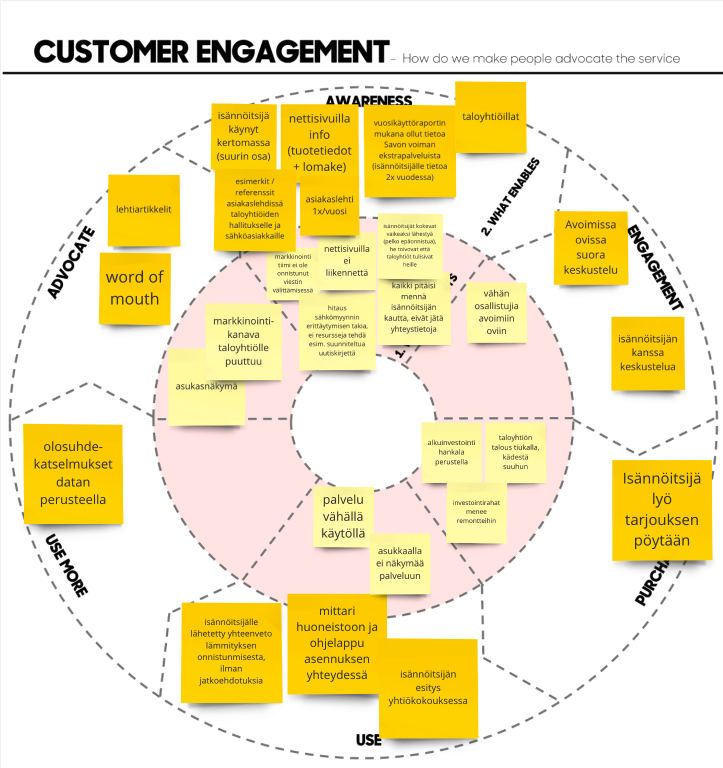
\includegraphics[width=\textwidth]{dippa/images/customer-engagement.png}
    \caption{Customer engagement canvas filled with one energy company}
    \label{fig:customer-engagement}
  \end{center}
\end{figure}

\subsubsection*{Awareness and Engagement Phases Overlap}

In the awareness phase, which is the first step, it depends on the energy company how they rise the awareness about the service. It is quite normal that the first time the housing company's chairperson hear about the service is when they receive an offer from the energy company. If that is the case, the offer usually has also some info material about the service. Another way for a housing company to know about the service is from the energy company's website where they have information about services and products that they offer. Additionally, the energy companies send newsletters and customer magazines to all of their customers where they inform their customers about new services or have some case stories featuring their services. However, it was clear that this way of doing is not that effective and it is left for the housing company board member's responsibility to then proceed with the topic.

During the awareness phase many problems were identified in addition to the previously mentioned. One issue was that the web pages do not have much of a traffic, so getting people for the right page is difficult. Moreover it was stated that marketing team should succeed to deliver the message to the customer. If the deputy landlord is responsible for discussing and also selling the service it was mentioned that they might deliver the message differently. This then leads to the situation where the energy company do not really know how the deputy landlords present the service. If the selling do not succeed the reasons behind the decision do not come into the knowledge of the energy companies. From the deputy landlords perspective, they might feel it is hard to approach the boards of the housing companies because they are afraid of failure and hope that they would approach them instead. 

Engagement is happening between the housing company board and energy companies only in rare situation. This is usually happening in open day events when the people have opportunity to discuss about the available services with the representative from the energy companies. Another form of engagement is a call after the offer is sent to discuss about the offered service more. However, it was discovered that these calls do not happen in every situations.

The main problem identified concern the fact that awareness and engagement phases are actually overlapping and there is no clear pattern or guidance on how the journey should go. Some energy companies are also lacking resources for example in marketing and then the responsibility for doing the communication is left for one person in the energy company. This leads then to the situation where closing the deals is not succeeding. Because of this it was also difficult to fill the steps after the purchase phase and the answers for them were mainly ideas how things could go if they were able to sell the service.

\section{Results from User Testing and Prototyping}

The following chapter will present the result gained from the the conducted experiments related to pricing model and personal selling. 

\subsection{Pricing Model}

In order to gain insights about pricing models and which of them is thought as the most suitable choice by the housing company's board members, the researcher and the team participated to housing company fair. There the fake ads were shown to 12 people. Eight of them were members of the board of a housing company, two were deputy landlords, one had background in housing company sales and one worked in a energy company.

Ten out of twelve people chose the pricing model that had the service fee which would be covered with the savings. Two out of twelve people did not have an opinion and three people said they would pick the investment pricing model if the housing company was wealthy otherwise the service fee with the savings.

\subsubsection*{Insights and Impact}

From this testing the biggest insight was that investment is not a good option to have as the only choice since the members of housing companies might fear to make a decision about it. However, if the housing company do have money on their account, the investment is the best option because in a long run it is more affordable.

As a result of the test, the partner company decided to move from an investment based pricing model to a pricing model which do not have investment and the service is paid with the saved costs. In addition, from this testing the case company also decided to have the service fee without investment as the main pricing model which they recommend for the partner companies.

In addition to the pricing model, the team received feedback about the advertisement and the texts in it. Related to showing the pricing, it was hoped by the test people to show price per apartment and not only for the building so it would be more understandable. Additionally, the contract period was hoped to be mentioned in the advertise. All in all the overall feedback was positive and the service was commented to be useful.

\subsection{Support for Personal Selling}

The researcher attended in a one open day event which was organised by one of the energy company partner. There the researcher was presenting the case company and working as a sales person for the energy company. The researcher approached people attending the open day with the customised offers which were done by the team for the specific housing companies.

\subsubsection*{Insights and Impact}

Attendance for an open day was not that great from the perspective of the housing companies. The researcher was able to speak only for three board members. The researcher gave the people the offer which also included the basic information about the service and let them read the paper. Afterwards, the researcher answered the questions and provided consultancy for the people if there were some unclear matters.

The researcher noticed that it was necessary to give a short presentation about the service in addition to the information which was presented in the paper. The board members were really interested in receiving the offer, because the researcher was able to give them a customized offer that stated the estimated savings in their housing company. In addition, the overall feedback about the service was positive.

